\clearemptydoublepage
\part*{Appendix}
\addcontentsline{toc}{chapter}{Appendix}
\label{p:appendix}


\chapter*{From Consul to Cheops: first tests on a dummy Cloud Application}
\label{chap:first-approach}

% Golic: In an insane world, a sane man must appear insane.

% \subsection{First version of Cheops: a static approach}

During 2021 spring, I supervised two interns, Matthieu Juzdzewski and Arnaud
Szymanek, worked on a first adaptation of our approach with the goal
of giving information on using a service mesh to implement the
theoritical approach given in~\autoref{chap:overview}.

In this first version, the idea was to have an entire instance of an
application on each site we want, and create a Cheops agent that would
also stand on each site.
%
These agents would be responsible to interpret the requests and
transfer them according to the \scl.
%
Also on each site, a reverse proxy besides every service, transferring
their requests to the local Cheops agent for interpretation.
%
% Agents communicate between each other and check each other status via
% heartbeats.
%
This implementation used Consul service
mesh\footnote{\url{https://www.consul.io/}} and
Envoy\footnote{\url{https://www.envoyproxy.io/}} as reverse proxy to
intercept and redirect, when needed, the requests.
%
% It is also worth noting that Envoy intercepts inbound and outgoing
% requests from services except for requests coming from Cheops agents.

The starting point for this work was we needed three components:
\begin{itemize}
\item intercepting/forwarding requests
\item knowledge of the services of the target application and their
  endpoints
\item extraction and interpretation of the scope in the requests
\end{itemize}

As it happens, a service mesh can execute the two first requirements,
the last needing to be implemented ourselves because it is \scl
specific.
%
As we discussed in~\autoref{chap:soa-SM}, Envoy works as a sidecar
proxy for every service and allowed for interception of requests.
%
Consul also uses a catalog that can be used dynamically to register
and unregister
services\footnote{\url{https://developer.hashicorp.com/consul/docs/discovery/services}
  - Accessed 2022-09-25}.

In this first version, there were two different components for Cheops:
the \emph{core} and the \emph{connector}.
%
The core received all requests to extract the scope, interpret where
to send the request and forward it.
%
If an address was local to the application instance (on the same
site), it used the Consul catalog to get the corresponding service
endpoint; otherwise, it was sent to the connector.
%
The connector was responsible to send a request on a distant host by
using a dictionary of known sites, and then the distant connector to
the corresponding service on its own site.

Unfortunately, with the complexity of the service mesh and proxy, this
work was working only on a simple use-case using two services
(ServiceA and ServiceB), which only purpose was for the first to call
for a resource on the second, to test if the sharing collaboration can
be achieved.
%
The original goal was to use Google Cloud Platform Online Boutique
Demo\footnote{\url{https://github.com/GoogleCloudPlatform/microservices-demo}},
but the purpose of this particular demo is to show the Anthos service
mesh usage, and thus was not really designed to manipulate the
resources inside.
%
This is why we deferred to two simple services with basic
functionalities and calls.
%
Moreover, in this version of Cheops, Envoy was configured to only
intercept and redirect requests for each service through a
ServiceRouter configuration.
%
Each service thus required a specific configuration to do so, and a
specific endpoint in Cheops.

\begin{figure}[htbp]
  \centering
  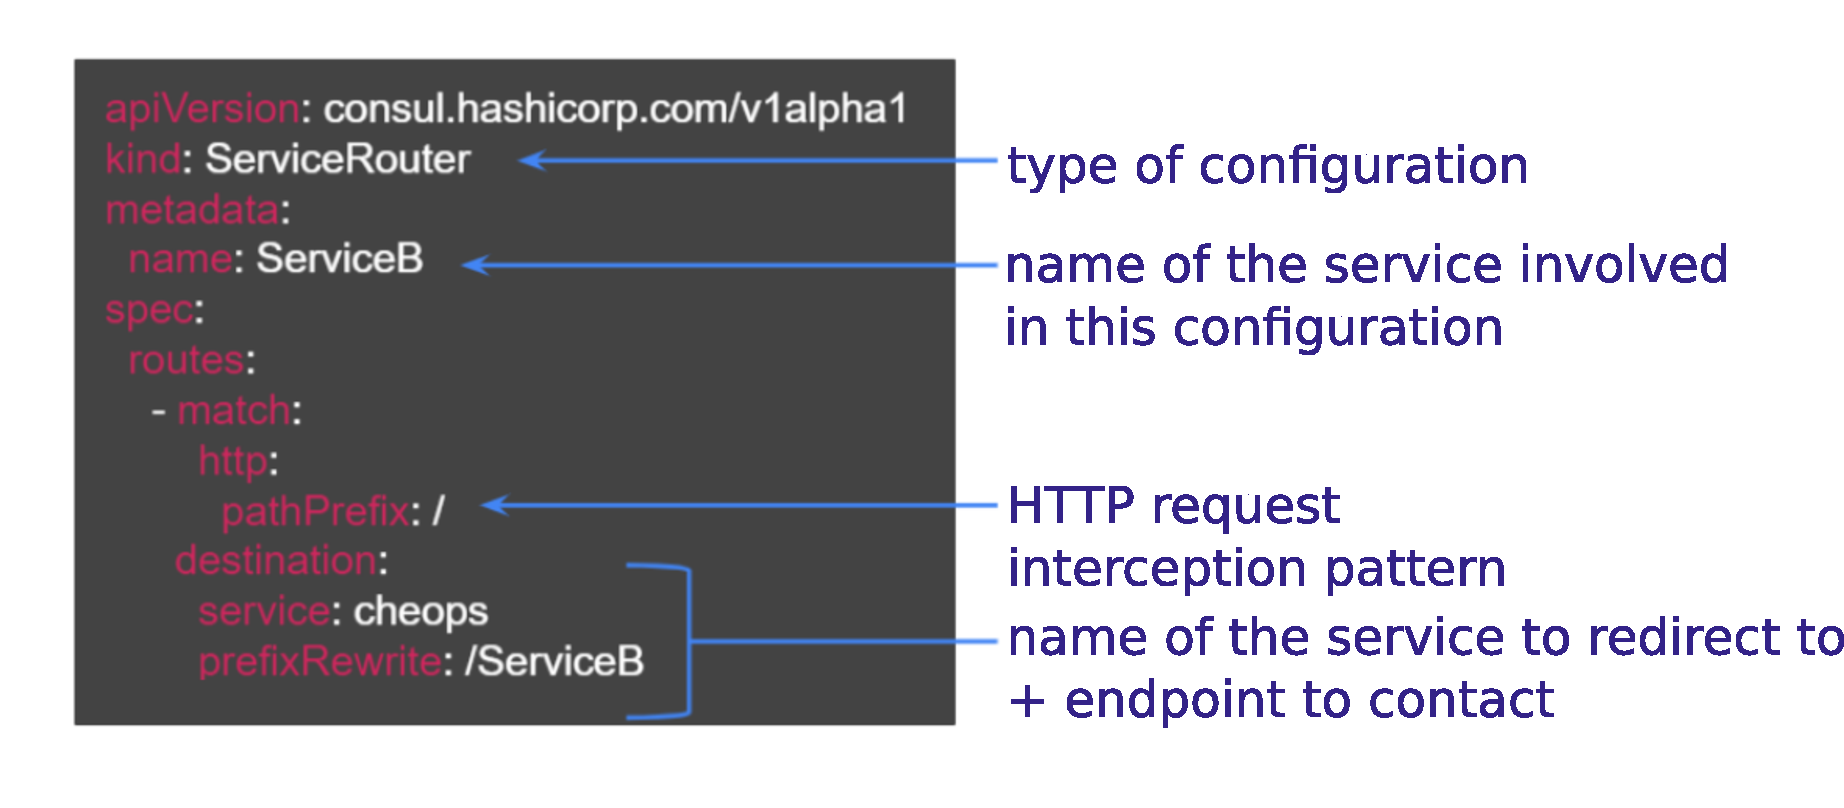
\includegraphics[width=\textwidth]{figs/pdf/cheopsv1-config}
  \caption{Configuration of a service in Envoy in the first version of Cheops.}
  \label{fig:cheops-v1-config}
\end{figure}

\autoref{fig:cheops-v1-config} shows the type of configuration that
was done to achieve the redirection to Cheops core.
%
For each ServiceB (metadata $\rightarrow$ name), every request will be
intercepted (the prefix is $/$), and will be redirected to the Cheops
service, at the endpoint \verb|/ServiceB|.
%
Thus, Envoy will redirect indiscriminately every request that comes
to ServiceB to Cheops for checking.


\begin{figure}[htbp]
  \centering
  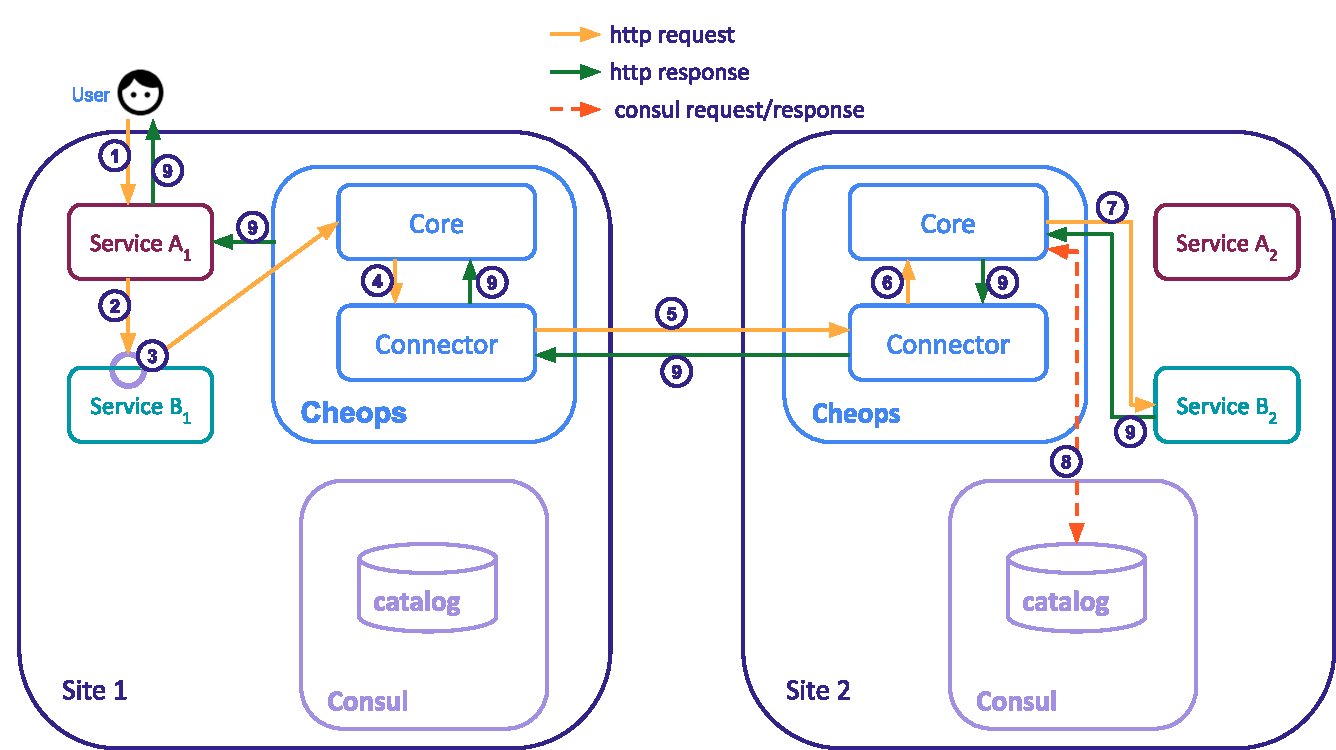
\includegraphics[width=\textwidth]{figs/pdf/cheopsv1}
  \caption{Workflow of a sharing request in the first version of Cheops.}
  \label{fig:cheops-v1}
\end{figure}

\autoref{fig:cheops-v1} presents the workflow of a request to use
$ServiceA_1$ and $ServiceB_2$, which means to use ServiceA on Site 1
and ServiceB on Site 2.
%
ServiceA has an endpoint $e$, which is called with an HTTP request:
\verb|http://address/ServiceA/e|.
%
ServiceB has an endpoint $h$, which is also called with an HTTP request:
\verb|http://address/ServiceB/h|.
%
This particular endpoint $h$ is the one called by ServiceA to execute
the workflow called with the endpoint $e$.
\begin{enumerate}
\item The request is made to use endpoint $e$ of ServiceA such as \\
  \verb|curl http://address/ServiceA/e -H "scope: ServiceB/Site2"|,
  with the scope thus integrated in the header.
\item To complete the workflow, ServiceA contacts the $h$ endpoint of
  ServiceB.
\item The prefix ``/h'' is recognized as an interception pattern for
  Envoy; the request is effectively intercepted and redirected to
  Cheops core on its /ServiceB endpoint.
\item The core extracts, interprets the scope and sends the request
  toward the connector since it cannot serve the request locally.
\item The connector finds in its registry the IP address for Site 2
  and transfers the request to Cheops connector on Site 2.
\item The connector on Site 2 redirects the request to its local core.
\item The core asks Consul catalog to get the address of the local
  ServiceB required; then finally transfers the request to this
  $ServiceB_2$.
\item The response from ServiceB is transferred back to $ServiceA_1$
  where the resource will be used to complete the workflow.
\end{enumerate}

This work on the first version of Cheops has been validated on two
different sites (Nantes and Rennes as Site 1 and Site 2) on the
Grid'5000 testbed~\cite{grid5000} (see~\autoref{fig:grid5000}).
%
The services have been deployed as Docker Containers through
Kubernetes.


\begin{figure}
  \centering
  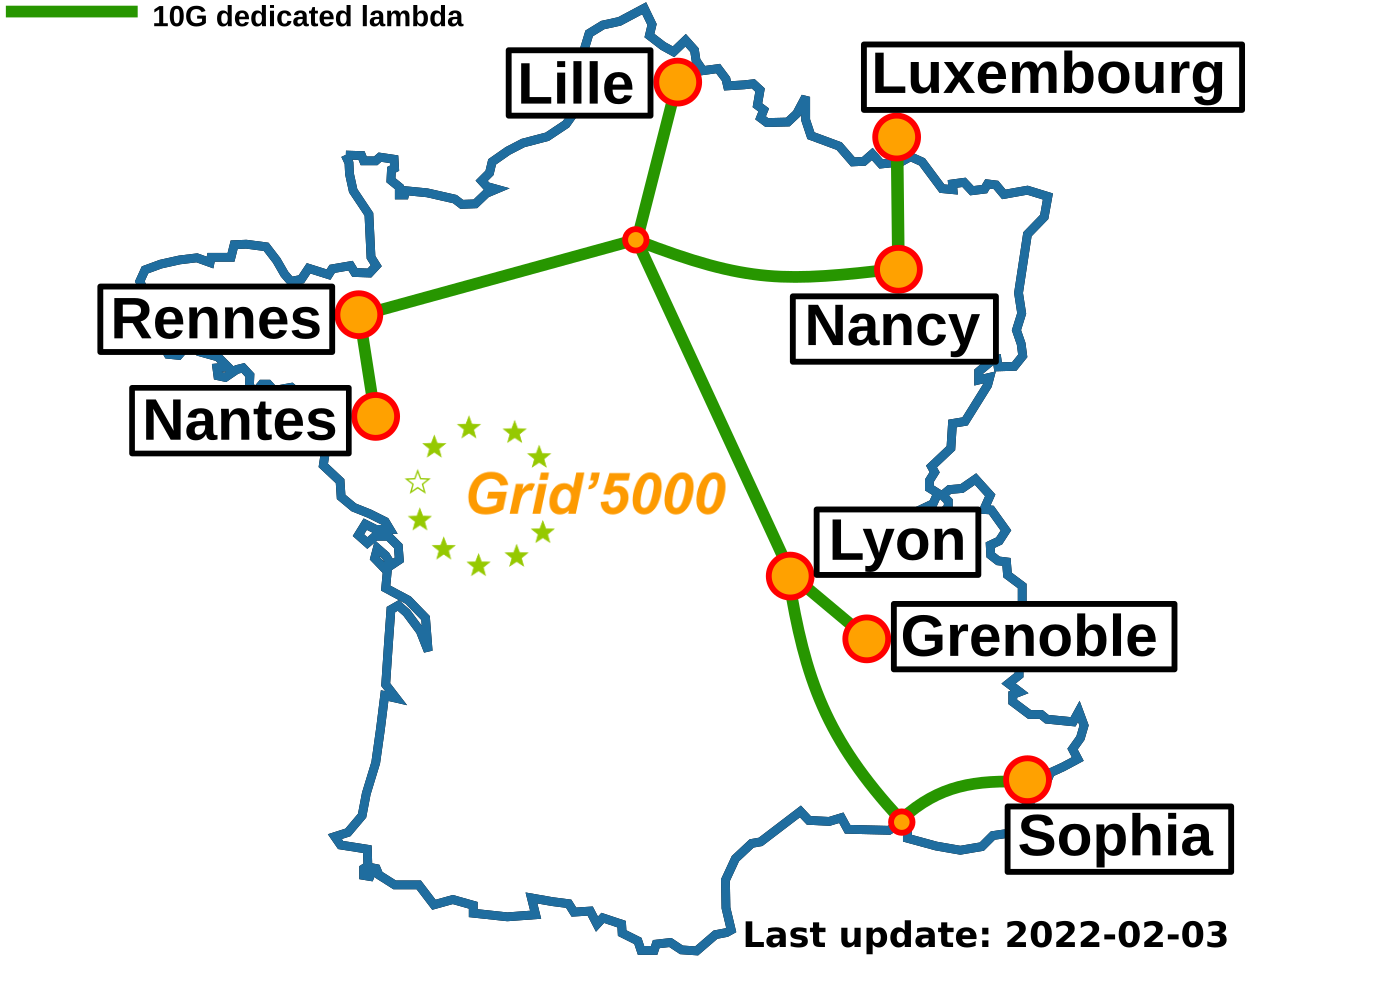
\includegraphics[width=.6\linewidth]{figs/png/Renater5-g5k.png}
  \caption{Grid'5000 and the Renater network.}
  \label{fig:grid5000}
\end{figure}

The experiment only showed it is possible to use a resource from
another site with sharing: ServiceA prints a string coming from
ServiceB.
%
The value of the string was ``I'm from Site 1'' on $ServiceB_1$ and
``I'm from Site 2'' on $ServiceB_2$.
%
The request sent to $ServiceA_1$ was:
\verb|curl http://localhost:1234/ServiceA/e -H "scope: ServiceB/Site2"|
and ServiceA printed ``I'm from Site 2''.

As mentioned, this version required an endpoint for every service
hard-coded in the Cheops core.
%
Moreover, Consul and Envoy had much more functionalities we did not
required, so we decided to do our own light service mesh.


This version of Cheops is available on the Cheops project
page\footnote{\url{https://gitlab.inria.fr/discovery/cheops/-/tree/v0.1.0}}.
